\documentclass[letterpaper]{article} % DO NOT CHANGE THIS
\usepackage[submission]{aaai2027}  % DO NOT CHANGE THIS
\usepackage[hyphens]{url}  % DO NOT CHANGE THIS
\usepackage{graphicx} % DO NOT CHANGE THIS
\urlstyle{rm} % DO NOT CHANGE THIS
\def\UrlFont{\rm}  % DO NOT CHANGE THIS
\usepackage{natbib}  % DO NOT CHANGE THIS AND DO NOT ADD ANY OPTIONS TO IT
\usepackage{caption} % DO NOT CHANGE THIS AND DO NOT ADD ANY OPTIONS TO IT
\frenchspacing  % DO NOT CHANGE THIS
\usepackage{amsmath}
\usepackage{amssymb}
\usepackage{amsthm}
\usepackage{booktabs}
\usepackage{placeins}
\newtheorem{proposition}{Proposition}
\pdfinfo{
/TemplateVersion (2027.1)
}
\setcounter{secnumdepth}{0}

\title{WEAVE: Wavelet-Routed Latent Style Transfer Trained in Minutes}
\author{
    Anonymous Submission
}
\affiliations{
}
\begin{document}
\maketitle

\begin{abstract}
Current style transfer methods are often ranked below a trivial identity mapping under commonly reported metrics such as LPIPS and ArtFID, which primarily reward content preservation. On direct style-similarity metrics, some spatial-domain models trained for hours even fall below this identity baseline. While state-of-the-art diffusion models and training-free methods built on them achieve stronger target-style transfer, their memory demands can exceed the VRAM limits of consumer GPUs. A natural lower-cost alternative is to learn compact transport in the compressed space of a frozen VAE. However, nonlinear, lossy encoding complicates appearance endpoints, while spectral bias allows low-frequency structural residuals to dominate optimization and suppress high-frequency style gradients.

We propose WEAVE, a compact wavelet-routed framework for VAE-latent transport. A single-level Haar transform separates the latent into frequency bands. A lightweight velocity model learns source-aligned LL transport together with LH/HL motion, while stepwise statistical alignment injects target-style statistics into the high-frequency bands, including HH, without changing the LL base. This learned--analytic split makes the remaining latent transport learnable by a compact field.

We further introduce the IDT--TGT sandwich, which brackets transfer between an identity floor and a source-independent target-style anchor. WEAVE clears the identity baseline in both CLIP-S and DINO-S, occupying a competitive position on the style--content Pareto frontier. With only 1.04M trainable parameters, it trains in 1.4 minutes after latent caching on a single RTX 3060, showing that its efficiency does not arise from identity-like under-transfer.
\end{abstract}

\begin{figure}[t]
\centering
\includegraphics[width=\columnwidth]{fig_page1_a.png}
\caption{Style--content trade-off on D5, with mean style affinity defined as $(\mathrm{CLIP\text{-}S}+\mathrm{DINO\text{-}S})/2$. Bubble area denotes task-specific training time for trainable methods; training-free methods use a fixed marker size. WEAVE exceeds IDT on both style metrics and reaches higher mean style affinity than the similarly content-preserving SaMam operating point, at substantially lower training cost.}
\label{fig:page1-a}
\end{figure}

\section{Introduction}

Recent diffusion and foundation-model editors provide strong priors for artistic style
transfer, but their computational cost remains prohibitive for consumer deployment. Systems
built on repeated diffusion denoising, inversion, or large image foundation models can
require tens of gigabytes of GPU memory and minutes to hours of
inference~\cite{wu2025qwenimagetechnicalreport,blackforestlabs2025flux2,chung2024style,hertz2024style,lu2024zstar}.
A natural route to lower cost is to perform transfer in the compressed space of a frozen
variational autoencoder, where spatial dimensions are smaller, representations can be
cached, and the remaining transport can in principle be modeled by a compact
network~\cite{rombach2022high}. Yet VAE compression introduces a less visible obstacle:
transformations that are simple in RGB space need not remain simple after nonlinear, lossy
encoding. \emph{VAE compression lowers spatial cost, but can make the transport itself
substantially harder to learn.}

Direct latent endpoints are both less affine and harder for a matched predictor to learn
than their pixel-space counterparts (Figure~\ref{fig:pixel-latent-affine}). Subband and
gradient measurements attribute this difficulty to low-frequency residuals from unrelated
reference geometry dominating high-frequency style motion.

We address this with \textbf{WEAVE}, a source-aligned, wavelet-routed latent flow that
separates learned low- and mid-frequency transport from analytic high-frequency style
injection: a compact velocity model predicts motion for the LL/LH/HL bands while stepwise
statistical alignment supplies the remaining high-frequency style
(Figure~\ref{fig:framework}). This observation is broader than style transfer: latent
representations optimized for reconstruction need not be compatible with low-capacity editing
or conditional transport. WEAVE turns the observation into a solver design: it removes
analytically tractable HF correction from the learned burden and reserves the compact field
for the remaining base and oriented residual motion.

A compact model can also obtain favorable content-oriented scores simply by staying close
to the input; we therefore evaluate WEAVE against an identity floor and a target-style copy
anchor (\textbf{IDT--TGT sandwich}) to confirm its efficiency does not come from
under-transferring. WEAVE clears the identity anchor under both DINO-S and CLIP-S while
retaining substantially more content than comparable diffusion editors, at 1.04M trainable
parameters and 1.4 minutes of training on a consumer GPU.

\paragraph{Contributions.}
Our contributions are threefold.
\begin{enumerate}
\item \textbf{Compact transport diagnosis.} We identify a compression--transport gap: VAE
compression reduces spatial cost but can make simple appearance transformations
substantially harder to learn. Endpoint residuals, matched convergence, and subband-gradient
measurements provide diagnostics of a latent representation's transport compatibility.
\item \textbf{Wavelet-routed affine-fiber transport.} WEAVE uses the Haar-induced
decomposition to assign source-aligned LL base motion, target-conditioned LH/HL
vertical motion, and fiber-preserving high-frequency statistical alignment. This learned--analytic
factorization makes residual latent transport learnable with a 1.04M-parameter field. The resulting
collection-level transport prior can further register a new style by updating only its
0.098M memory entry.
\item \textbf{Valid transfer at minute-scale cost.} We introduce the IDT--TGT sandwich to
verify that computational savings do not arise from identity-like behavior. WEAVE clears
the identity anchor, occupies a competitive style--content Pareto position, and---restricted
to sandwich-valid methods with fully reported timing---delivers about a $5\times$ lower
end-to-end train+infer cost (counting the one-time latent-caching pass) than the fastest such baseline on the 750-image board.
\end{enumerate}

\section{Related Work}
\label{sec:related}

Classical NST replaces iterative optimization with feed-forward, attention-based, or style-bank transforms~\cite{gatys2015neural,gatys2016image,huang2017arbitrary,li2017universal,park2019sanet,deng2022stytr2,hong2023aespa,kwon2024aesfa,park2020cut,gim2024cast,zhang2024s2wat,zhang2025survey,chen2017stylebank}. Unlike style-specific transformation banks, WEAVE uses memory only as a coarse prior and derives exemplar-specific conditioning from routed HF codes and moments.

Diffusion editors also act in frozen-VAE latents but still invoke a large denoiser at inference~\cite{rombach2022high,hertz2022prompt,meng2021sdedit,chung2024style,hertz2024style,ye2023ipadapter,zhang2023inst,kim2022diffuseit,zhang2024artbank,lu2024zstar,wu2025qwenimagetechnicalreport,blackforestlabs2025flux2}. WEAVE keeps the frozen VAE but removes the diffusion U-Net from transport, using a compact field plus an analytic update (validated as an SD1.5 plug-in).

Flow-matching and Schr\"odinger-bridge methods learn transport between endpoint distributions~\cite{liu2022rectified,lipman2022flow,leonard2014survey,debortoli2021dsb,shi2023dsbm,liu2023i2sb,su2023ddib,cuturi2013sinkhorn,peyre2019computational}. Recent latent variants reduce inference cost: LBM learns a latent bridge for fast image-to-image translation~\cite{chadebec2025lbm}, and Latent Schr\"odinger Bridge reuses pretrained diffusion predictors to approximate unpaired transport with fewer evaluations~\cite{kim2024latentsb}. WEAVE keeps flow-matching supervision but reformulates exemplar-conditioned style endpoints and assigns each solver step a fiber-preserving analytic operator; its contribution is the learned--analytic responsibility split, not a new bridge objective.

Mamba-based state-space models give global receptive fields at linear cost for style transfer~\cite{gu2023mamba}: SaMam~\cite{liu2024samam} uses a style-aware Mamba encoder--decoder over flattened spatial tokens without decomposing frequency subbands, while SaMST~\cite{liu2024samst} decouples style learning from a compact convolutional transfer network. WEAVE instead decomposes the latent into an orthonormal Haar basis and routes LL/LH/HL to separate lightweight heads, reserving HH for analytic alignment---without a sequential backbone, a token-domain design, or a diffusion U-Net.
\begin{figure}[t]
\centering
\includegraphics[width=\columnwidth]{fig_page1_b.png}
\caption{ArtFID vs.\ style affinity $(\mathrm{CLIP\text{-}S}+\mathrm{DINO\text{-}S})/2$ on D5 ($r(\mathrm{style},-\mathrm{ArtFID})=-0.68$). On D5, ArtFID favors strongly content-preserving operating points, including identity, and therefore should not be interpreted as a standalone ranking of style strength.}
\label{fig:page1-b}
\end{figure}
\begin{figure*}[t]
\centering
\includegraphics[width=\textwidth]{frame.png}
\caption{WEAVE architecture. At each of the $K=8$ steps, a compact field updates LL/LH/HL; $S_s$ then aligns HF statistics while preserving the updated LL base (no learned HH head). Style memory $m_s$ is a learned lookup for registered style ID $s$; the target exemplar supplies pooled LH/HL codes to the learned routes and HF moments to $S_s$. Bottom: training-only endpoint and routed loss.}
\label{fig:framework}
\end{figure*}
LPIPS and ArtFID may reward content-preserving near-copies~\cite{zhang2018unreasonable,wright2022artfid}, and no single metric captures both style affinity and content fidelity~\cite{ioannou2024evaluation}. On D5, style affinity correlates negatively with $-\mathrm{ArtFID}$ ($r=-0.68$, Figure~\ref{fig:page1-b}); we therefore report style and content separately and use the IDT--TGT sandwich as a validity frame rather than a style-strength ranking.





Spectral-bias and frequency-aware models separate scales in objectives or generation heads~\cite{rahaman2019spectral,xu2022frequency,cai2021fdit,ren2026freqflow}; wavelets give exact multi-band coordinates~\cite{phung2023wavelet,yoo2019photorealistic,daubechies1992ten}. Prior work uses wavelets for compression, high-resolution supervision, or one-shot style initialization~\cite{sadat2024litevae,sigillo2025latentwavelet,zhang2025diffusion4k,wang2025dgpst}; DGPST applies AdaIN--Wavelet initialization after semantic warping, whereas WEAVE routes learned LL/LH/HL motion with stepwise analytic HF alignment inside the solver, without a diffusion denoiser. Frequency-aware tokenizers such as the FA-VAE variants improve reconstruction by preserving or decoupling high-frequency information~\cite{lin2023favae,yin2025favae}; WEAVE is complementary, freezing the tokenizer and asking whether the resulting latent geometry supports low-capacity conditional transport, which reconstruction fidelity alone does not determine.


\section{Method}
\label{sec:method}

WEAVE formulates style transfer as wavelet-routed transport in VAE latent space
(Figure~\ref{fig:framework}): it source-aligns the LL endpoint, assigns LL/LH/HL motion to a
compact velocity field, and handles the remaining high-frequency statistics analytically.



\subsection{Why Direct Latent Transport Is Difficult}
\label{sec:why-hard}

For an RGB map $T$, the normalized residual of the best pointwise affine fit is
\begin{equation}
\begin{aligned}
R_q(T)&=\min_{A,b}
\frac{\|Aq(x_c)+b-q(T(x_c,x_s))\|_2^2}
{\|q(T(x_c,x_s))-q(x_c)\|_2^2},\\
&\qquad q\in\{I,\mathcal E\}.
\end{aligned}
\label{eq:affine-representability}
\end{equation}
Figure~\ref{fig:pixel-latent-affine} shows $R_{\mathcal E}\!\gg\!R_I$ for color shift,
AdaIN, WCT, and gamma maps, and a matched TinyUNet (same width; pixel at $256^2$, latent at
$32^2$) converges far more slowly on direct latent endpoints than on pixel or
frequency-structured latent endpoints. Shared MSE then lets low-frequency residuals from
unrelated reference geometry dominate the
update~\cite{rahaman2019spectral,xu2022frequency,cai2021fdit}. \emph{We therefore
reformulate the transport before increasing capacity.}

\begin{figure}[t]
\centering
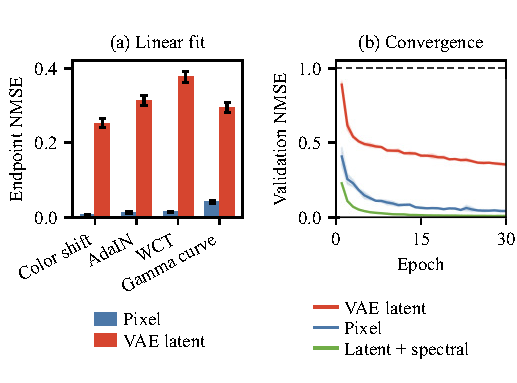
\includegraphics[width=\columnwidth]{fig_pixel_vs_latent_one_column.pdf}
\caption{Pixel vs.\ VAE-latent endpoint fit. (a)~Affine residual. (b)~Matched
TinyUNet: frequency-structured latents recover learnability.}
\label{fig:pixel-latent-affine}
\end{figure}

\subsection{Haar-Induced Affine-Fiber Coordinates}
\label{sec:wavelet}

A one-level orthonormal Haar map $\mathcal W(z)=(\ell,h_1,h_2,h_3)$ exposes LL and oriented
HF bands~\cite{daubechies1992ten}. With $P_Lz=\mathcal W^{-1}(\ell,0,0,0)$, $P_H{=}I{-}P_L$,
and $\pi_L(z){=}\ell$, the fiber over $\ell$ is the exact affine set
\begin{equation}
\mathcal F_{\ell}=\pi_L^{-1}(\ell)
=\mathcal W^{-1}(\ell,0,0,0)+\ker P_L,
\label{eq:affine-fiber}
\end{equation}
Thus $\mathcal Z=\operatorname{im}P_L\oplus\ker P_L$. We use ``affine fiber'' only in the
linear sense of Eq.~\ref{eq:affine-fiber}: an operator coordinate split, not a semantic
content/style partition. LL may still contain style, and HF may contain geometric edges.


\subsection{Source-Aligned LL Endpoint}
\label{sec:framework}

Let $z_c{=}\mathcal E(x_c)$ and $z_s{=}\mathcal E(x_s)$ from the frozen SD1.5
VAE~\cite{rombach2022high}. Direct $z_c{\to}z_s$ supervises unrelated base geometry in
$\ell_s$. WEAVE replaces the base destination by
\begin{equation}
\begin{aligned}
\tilde\ell_s &=(1-\alpha)\ell_c+
\alpha\,\mathrm{AdaIN}(\ell_c,\ell_s),\qquad \alpha=0.3,\\
z_1^\star&=\mathcal W^{-1}(\tilde\ell_s,h_{1,s},h_{2,s},h_{3,s}),
\end{aligned}
\label{eq:aligned-target}
\end{equation}
keeping target HF coordinates. Training uses a lightly noised rectified path
\begin{equation}
z_t=(1-t)z_c+t z_1^\star-\sigma\sqrt{t(1-t)}\,\epsilon,\qquad
u=z_1^\star-z_c,
\label{eq:rf-path}
\end{equation}
with $t{\sim}\mathcal U([0,1])$, $\epsilon{\sim}\mathcal N(0,I)$, $\sigma{=}0.02$;
supervision is the clean displacement $u$ (noise off at inference).

\subsection{Learned Base and Vertical Transport}
\label{sec:sfm}

The field predicts only base and LH/HL vertical velocities,
\begin{equation}
v_\theta(z_t,t,s)=(v_\ell,\,v_{h_1},\,v_{h_2},\,0),
\label{eq:velocity-split}
\end{equation}
Because $\mathcal W$ is orthonormal, Parseval gives an exact subband decomposition of any
latent residual:
\begin{equation}
\begin{aligned}
\|z{-}z'\|_2^2
&=\|\ell{-}\ell'\|_2^2
+\|h_1{-}h_1'\|_2^2 \\
&\quad+\|h_2{-}h_2'\|_2^2
+\|h_3{-}h_3'\|_2^2.
\end{aligned}
\label{eq:parseval}
\end{equation}
Under a shared MSE on $z$, a large LL residual can dominate the total
gradient and starve the HF heads. Subband routing makes this
frequency-scale imbalance explicit and controllable: spectral matching
with $\lambda_{LL}{=}0.3$ (results remain stable at $1.0$; Table~\ref{tab:ablation})
\begin{equation}
\mathcal L_{\mathrm{SFM}}
=\mathbb E_t\big[
\lambda_{LL}\|v_\ell-u_\ell\|_2^2
+\|v_{h_1}-u_{h_1}\|_2^2
+\|v_{h_2}-u_{h_2}\|_2^2\big]
\label{eq:weave-loss}
\end{equation}
weights LL explicitly, while HH never enters the learned gradient (analytic path only).
A width-64 residual trunk with separate $1{\times}1$ LL/LH/HL heads implements $v_\theta$;
no HH head is learned. Style enters through one learned $256\times384$ memory entry per registered style. Reference exemplars independently provide pooled LH/HL codes to the learned routes and HF moments to $S_s$. Unseen styles clamp the memory path but retain both reference-derived routes. Registration appends a new memory entry and optimizes only its 0.098M parameters while freezing the remaining model (Table~\ref{tab:register}).

\subsection{Fiber-Preserving Statistical Alignment}
\label{sec:eota}

For $q{=}P_H(z)$ and $q_s{=}P_H(z_s)$, channel-wise AdaIN~\cite{huang2017arbitrary}
\begin{equation}
\mathcal A(q;q_s)=
\frac{q-\mu(q)}{\sigma(q)+\varepsilon}\,\sigma(q_s)+\mu(q_s)
\label{eq:spatial-fiber-adain}
\end{equation}
defines the fiber-preserving map
\begin{equation}
\begin{aligned}
S_s(z)&=P_L z+\Psi_s(P_H z),\\
\Psi_s(q)&=(1-\beta)q+\beta\,\mathcal A\!\bigl(q;(1+\eta)q_s\bigr).
\end{aligned}
\label{eq:fiber-operator}
\end{equation}
Because $q=P_Hz=\mathcal W^{-1}(0,h_1,h_2,h_3)$ is the reconstructed HF residual, each local Haar block has zero mean. Hence $\mu(q)=\mu(q_s)=0$ and
\[
\mathcal A(q;q_s)
=
q\cdot\frac{\sigma(q_s)}{\sigma(q)+\varepsilon},
\]
which remains a channel-wise scaling in $\ker P_L$.

\begin{proposition}[Base preservation]
\label{prop:base-preserve}
$\pi_L(S_s(z))=\pi_L(z)$ for all $z$, i.e.\ $S_s:\mathcal F_\ell\to\mathcal F_\ell$.
\end{proposition}
\begin{proof}
$P_H z\in\ker P_L$ and the scaling property of $\mathcal A$ imply
$\Psi_s(P_H z)\in\ker P_L$, so
$\pi_L(S_s(z))=\pi_L(P_L z)=\pi_L(z)$.\qed
\end{proof}
Thus $S_s$ injects HF statistics (and supplies HH) without moving the current LL base;
applying it after every Euler step makes alignment part of the dynamics, not post-processing.

\subsection{Learned--Analytic Split Solver}
\label{sec:efficiency}

Inference alternates a learned Euler step and $S_s$:
\begin{equation}
z^{k+1}=S_s\circ\Phi_\theta^{1/K}(z^k),\qquad k=0,\dots,K-1,
\label{eq:split-solver}
\end{equation}
with $K{=}8$. Training minimizes Eq.~\ref{eq:weave-loss} on cached latents; the model has
$1.04$M trainable parameters plus the frozen $84$M VAE. Details are in the supplement.



\section{Experiments}
\label{sec:exp}

\begin{table*}[t]
\centering
{\small
\setlength{\tabcolsep}{1mm}
\begin{tabular}{@{}lcccccccccccccc@{}}
\toprule
& \multicolumn{4}{c}{D5-512}
& \multicolumn{4}{c}{P2A-256}
& \multicolumn{4}{c}{R5-WikiArt}
& Params & Train/Infer \\
\cmidrule(lr){2-5}\cmidrule(lr){6-9}\cmidrule(lr){10-13}\cmidrule(lr){14-14}\cmidrule(lr){15-15}
Method
& D-S & C-S & LP$\downarrow$ & D-C
& D-S & C-S & LP$\downarrow$ & D-C
& D-S & C-S & LP$\downarrow$ & D-C
& M & min \\
\midrule
IDT & 0.419 & 0.640 & 0.000 & 1.000 & 0.356 & 0.618 & 0.000 & 1.000 & 0.433 & 0.731 & 0.000 & 1.000 & 0 & --/-- \\
TGT & 1.000 & 0.855 & 0.756 & 0.220 & 1.000 & 0.835 & 0.800 & 0.169 & 1.000 & 0.796 & 0.747 & 0.230 & 0 & --/-- \\
SD-Turbo & 0.484 & 0.693 & \underline{\underline{\textbf{0.003}}} & \underline{\underline{\textbf{0.922}}} & 0.341$^{\dagger}$ & 0.674 & 0.603 & 0.279 & 0.505 & 0.767 & 0.449 & 0.538 & 0$^{+1100}$ & free/5 \\
StyleAligned & \underline{\underline{\textbf{0.675}}} & 0.780 & 0.869$^{\ddagger}$ & 0.239 & \underline{\underline{\textbf{0.612}}} & 0.768 & 0.786 & 0.310 & \underline{\underline{\textbf{0.649}}} & \underline{\underline{\textbf{0.824}}} & 0.829$^{\ddagger}$ & 0.315 & 0$^{+1100}$ & free/77 \\
Z-STAR & 0.449 & 0.784 & 0.347 & 0.549 & 0.514 & \underline{\underline{\textbf{0.786}}} & 0.332 & 0.526 & 0.514 & \underline{\textbf{0.822}} & 0.384 & 0.526 & 0$^{+1100}$ & free/180 \\
StyleShot & \underline{\textbf{0.563}} & \underline{\textbf{0.787}} & 0.765$^{\ddagger}$ & 0.377 & \underline{\textbf{0.552}} & \underline{\textbf{0.774}} & 0.713 & 0.335 & 0.484 & 0.787 & 0.795$^{\ddagger}$ & 0.380 & 0$^{+2400}$ & free/306 \\
StyleID & 0.548 & \underline{\underline{\textbf{0.822}}} & 0.552 & 0.416 & 0.256$^{\dagger}$ & 0.648 & 0.691 & 0.147$^{\ddagger}$ & \underline{\textbf{0.571}} & 0.815 & 0.493 & 0.374 & 0$^{+1100}$ & free/63 \\
CUT & 0.471 & 0.714 & 0.374 & 0.795 & 0.539 & 0.754 & 0.494 & 0.702 & 0.441 & 0.710$^{\dagger}$ & 0.620 & \underline{\textbf{0.795}} & 7.0 & 323/5 \\
SaMST & 0.271$^{\dagger}$ & 0.618$^{\dagger}$ & 0.749 & 0.145$^{\ddagger}$ & 0.501 & 0.709 & 0.398 & 0.838 & 0.461 & 0.667$^{\dagger}$ & 0.612 & 0.615 & 8.3 & 39.5/10 \\
SaMam & 0.477 & 0.702 & \underline{\textbf{0.248}} & \underline{\textbf{0.812}} & 0.505 & 0.677 & \underline{\underline{\textbf{0.205}}} & \underline{\underline{\textbf{0.870}}} & 0.503 & 0.712$^{\dagger}$ & \underline{\underline{\textbf{0.227}}} & \underline{\underline{\textbf{0.925}}} & 8.8 & 436/17.6 \\
StyTR-2 & 0.501 & 0.709 & 0.596 & 0.747 & 0.515 & 0.722 & 0.495 & 0.555 & 0.533 & 0.759 & 0.553 & 0.737 & 35$^{+13}$ & 1440/38 \\
AesPA-Net & 0.520 & 0.724 & 0.548 & 0.601 & 0.498 & 0.744 & 0.571 & 0.522 & 0.545 & 0.782 & 0.409 & 0.728 & 11$^{+20}$ & 6.1/23 \\
Seedream & 0.486 & 0.720 & 0.477 & 0.739 & 0.517 & 0.752 & \underline{\textbf{0.227}} & 0.785 & 0.504 & 0.742 & 0.486 & 0.725 & -- & API/-- \\
Latent-WCT & 0.362$^{\dagger}$ & 0.673$^{\dagger}$ & 0.441 & 0.559 & 0.338$^{\dagger}$ & 0.738 & 0.585 & 0.386 & 0.414$^{\dagger}$ & 0.710$^{\dagger}$ & 0.444 & 0.553 & 0$^{+84}$ & free/3.67 \\
\midrule
\textbf{WEAVE} & 0.492 & 0.713 & 0.259 & 0.810 & 0.480 & 0.668 & 0.312 & \underline{\textbf{0.861}} & 0.523 & 0.775 & \underline{\textbf{0.290}} & 0.772 & \underline{\underline{\textbf{1.04$^{+84}$}}} & \underline{\underline{\textbf{1.4/1.22}}} \\
\bottomrule
\end{tabular}
}
\caption{Main comparison ($\uparrow$/$\uparrow$/$\downarrow$/$\uparrow$ for D-S/C-S/LP/D-C). Best two non-anchor results are bold; double underline marks the best. $\dagger$: the style metric does not exceed its IDT value;
$\ddagger$: the content metric falls beyond the TGT reference. Params are in millions, with frozen parameters shown as superscripts; Train/Infer gives training and inference time in minutes for 750 outputs on an RTX 3060 unless noted. Trainable baselines use the same D5 split and evaluation board.}
\label{tab:main}
\end{table*}


\subsection{Implementation Details}
\label{sec:setup}

\paragraph{Datasets.}
All benchmarks are built from publicly available WikiArt images.
D5 uses the five WikiArt families whose identity/target-style CLIP-S gap is largest (Early Renaissance, Impressionism, Minimalism, Rococo, Ukiyo-e). Training uses 5,000 images (1,000 per family) and testing uses 150 images (30 per family); each test image is paired with one reference from every family, yielding 750 content--style pairs at $512\times512$ resolution.
P2A is the standard photo-to-art benchmark evaluated at $256\times256$.
To control for the CLIP-gap-based selection of D5, R5-WikiArt uses five styles drawn at random
from WikiArt (Cubism, Expressionism, Pop Art, Romanticism, Symbolism). As on D5, each of the
150 content images is paired with one reference from every family, yielding 750 pairs at
$512\times512$. It is distinct from Other5 below (a different five-family held-out set used
for zero-shot conditioning and memory-registration experiments).
For each request, the source content image and a target-style reference image are given; the task is to render the content in the target style.

\paragraph{Metrics.}
DINO-S measures target-style affinity as the maximum cosine similarity between DINOv2~\cite{oquab2023dinov2} CLS embeddings of the generated image and the CLS embeddings of the target-style reference pool (up to 30 reference images per style), following the standard photo-to-art evaluation protocol.
CLIP-S reports the cosine similarity between CLIP~\cite{radford2021clip} image features of the generated image and a target-style prototype formed as the L2-normalized mean CLIP feature over a fixed 16-image reference pool per style; the prototype is precomputed once per target style and shared across all 750 requests, so CLIP-S measures absolute style affinity rather than similarity to a particular reference image.
LPIPS measures perceptual content distance between the generated image and the source content image~\cite{zhang2018unreasonable}.
DINO-C reports DINOv2 cosine similarity between the generated image and the source, giving a complementary content-preservation view.
IDT (identity transfer) and TGT (target-style copy) are dataset-specific anchors: IDT returns the unchanged source image (no-op floor), while TGT returns a target-style reference as the opposite extreme (high style affinity, low content). They are empirical anchors, not mathematical bounds.
IDT/TGT are evaluated using the same metric-specific reference protocol as the methods they bracket (D5: 750 pairs; P2A IDT: cross-style transfer pairs with LPIPS${=}0$ and DINO-C${=}1$ by construction).
We mark methods that do not exceed IDT on style ($\dagger$) or fall outside TGT on content ($\ddagger$) in Table~\ref{tab:main}.

\paragraph{Configuration.}
Training uses $\alpha{=}0.3$, $\lambda_{LL}{=}0.3$, and $\sigma{=}0.02$ with evaluation-free internal stopping. Inference uses $\beta{=}2.0$, $\eta{=}0.1$, and $K{=}8$ across all boards; complete sensitivity results are provided in the supplement.

\paragraph{Baseline training protocol.}
Trainable baselines use the same D5 split and 750-pair evaluation board; timings are measured on RTX~3060-class hardware where available. Training-free editors use frozen public checkpoints or API outputs. D5, P2A, and R5 use collection-specific WEAVE models with shared solver defaults.

\subsection{Comparison with State-of-the-Art Methods}
\label{sec:sota}

\begin{figure*}[t!]
\centering
\includegraphics[width=\textwidth]{teaser.png}
\caption{High-content cross-domain transfer from Minimalism to Rococo.
Several baselines remain close to identity, whereas some diffusion
editors alter the source structure. WEAVE preserves the source topology
while shifting local color and texture toward the target, illustrating
the operating point quantified by the IDT--TGT analysis.}
\label{fig:teaser}
\end{figure*}

\paragraph{D5 quality--compute operating point.}
WEAVE clears IDT on both style metrics and reaches higher mean style
affinity than SaMam at similar content fidelity, with 1.04M trainable
parameters and substantially lower train/infer cost. Editors with
higher raw style affinity incur considerably larger content loss, as
contextualized by TGT. D5 uses the oriented target-HF route; P2A and R5
retain the same Haar/endpoint/stepwise-alignment factorization with the
base architecture.

\paragraph{Reading the sandwich.}
IDT identifies identity-like under-transfer, whereas TGT marks
target-copy-like content loss. WEAVE clears both IDT style anchors
without approaching TGT content loss; StyleAligned attains higher
DINO-S but crosses the TGT reference in LPIPS.

\paragraph{P2A and R5.}
WEAVE remains inside the IDT--TGT bracket on P2A. On R5, it improves
DINO-S over IDT, CUT, and SaMam while preserving more content than
StyTR-2 and AesPA-Net, supporting the same operating point beyond the
CLIP-gap-selected D5 styles.

\paragraph{Cost.}
Latent caching, training, and 750-image inference take approximately
3.0, 1.4, and 1.2 minutes, respectively, giving a 5.6-minute first-run
budget on one RTX~3060. Under the same five-style protocol, this is
about $10\times$ lower than StyleID's inference-only cost and
$80\times$ lower than our SaMam retrain's train+infer cost. The complete
pipeline fits within 12\,GB VRAM.

\subsection{Ablation Study}
\label{sec:ablation}

Table~\ref{tab:ablation} reports a transport-responsibility ablation: each variant removes
or reassigns one responsibility in Align--Route--Assign. Source alignment matters most for
content: replacing it with a direct target endpoint increases LPIPS by $0.05$ while leaving
DINO-S nearly unchanged. HF conditioning and stepwise AdaIN each independently contribute
to style affinity; final-only AdaIN collapses content. Pure $S_s$ supplies most style movement; the learned field adds
further style affinity and carries the LL and oriented residual motion. A learned HH head and $\lambda_{LL}{=}1.0$ give only
marginal changes, motivating the simpler default.

Per-step diagnostics confirm that $S_s$ supplies the dominant HF motion while the learned field carries LL and smaller oriented residual motion; full trajectories are provided in the supplement.



\begin{table}[ht]
\centering
\begin{tabular}{@{}lcccc@{}}
\toprule
Variant & D-S$\uparrow$ & C-S$\uparrow$ & LP$\downarrow$ & D-C$\uparrow$ \\
\midrule
\textbf{WEAVE} & 0.492 & 0.713 & 0.259 & 0.810 \\
w/o AdaIN & 0.482 & 0.701 & 0.226 & 0.846 \\
final-only AdaIN & 0.484 & 0.729 & 0.395 & 0.666 \\
w/o HF cond. & 0.483 & 0.716 & 0.284 & 0.813 \\
$\lambda_{LL}{=}1.0$ & 0.491 & 0.718 & 0.263 & 0.787 \\
direct endpoint & 0.489 & 0.717 & 0.314 & 0.797 \\
learned HH & 0.493 & 0.716 & 0.267 & 0.806 \\
zero velocity & 0.475 & 0.703 & 0.258 & 0.856 \\
\bottomrule
\end{tabular}
\caption{Ablation on 750 D5 pairs. Zero-velocity disables the learned field (pure $S_s$).}
\label{tab:ablation}
\end{table}

\subsection{Generalization and Robustness}
\label{sec:generalization}

We test the formulation across random seeds, VAE representations, held-out style families,
and a frozen editor.

\paragraph{Multiple seeds.}
The evaluation-free stopping rule selects epochs 4, 4, and 3 for seeds
42, 7, and 123. On a fixed latent probe, it stops at the first target-HF
gate expansion accompanied by at least a 35\% contraction of the
shared-trunk LL/HF gradient-norm ratio; no decoded image or
image-quality metric is used. Algorithm~S1 gives the complete rule.

\paragraph{Representation robustness.}
Table~\ref{tab:vae-port} replaces the frozen SD1.5 EMA VAE with FLUX.1, FLUX.2, and
Qwen-Image, retaining the same one-level Haar-routed factorization and evaluation-free
internal-dynamics selection, adapting channel projections to each latent width, and using
the learned-HH portability variant described in the supplement. All three clear IDT on style
with competitive content; FLUX.2 matches SD1.5 DINO-S while improving CLIP-S, LPIPS, and
DINO-C. \emph{The factorization is not tied to one tokenizer}, though the selected epoch
shifts with latent geometry. We retain Haar for orthogonality and cost.

\begin{table}[ht]
\centering
{\small
\setlength{\tabcolsep}{3.5pt}
\begin{tabular}{@{}lcccc@{}}
\toprule
Frozen VAE & D-S$\uparrow$ & C-S$\uparrow$ & LP$\downarrow$ & D-C$\uparrow$ \\
\midrule
SD1.5 EMA (main) & 0.492 & 0.713 & 0.259 & 0.810 \\
FLUX.1 & 0.489 & 0.713 & 0.256 & 0.780 \\
FLUX.2 & 0.492 & 0.717 & 0.239 & 0.873 \\
Qwen-Image & 0.478 & 0.714 & 0.263 & 0.825 \\
\bottomrule
\end{tabular}
}
\caption{Cross-VAE D5 under internal-dynamics selection (same evaluation-free rule as
SD1.5; SD1.5 is seed-42 main).}
\label{tab:vae-port}
\end{table}

\paragraph{Conditioning generalization.}
Across resampled reference pools, WEAVE retains a positive board-level
DINO-S margin over IDT. On the five held-out Other5 families, the D5
checkpoint gives the best CLIP-S and content metrics, while SaMam is
0.015 higher in DINO-S (Table~\ref{tab:ooze}), showing that the
reference-conditioned path generalizes beyond the registered style IDs.

\begin{table}[ht]
\centering
{\small
\begin{tabular}{@{}lcccc@{}}
\toprule
Method & D-S$\uparrow$ & C-S$\uparrow$ & LP$\downarrow$ & D-C$\uparrow$ \\
\midrule
WEAVE & 0.5313 & \textbf{0.7742} & \textbf{0.2802} & \textbf{0.7587} \\
SaMam & \textbf{0.5466} & 0.7577 & 0.3990 & 0.7369 \\
SaMST & 0.3913 & 0.7485 & 0.6213 & 0.2680 \\
\bottomrule
\end{tabular}
}
\caption{Zero-shot transfer on Other5 using the D5 checkpoint with the style-ID path
clamped. All five target families are held out from D5 (750 pairs).}
\label{tab:ooze}
\end{table}

\paragraph{Memory-only style registration.}
Starting from the D5 checkpoint, we append five Other5 entries and
optimize only their 0.49M parameters for 3{,}000 steps. Registration
takes 98\,s, improves all four metrics over zero-shot, and matches
full-field fine-tuning within 0.003 DINO-S and 0.001 CLIP-S
(Table~\ref{tab:register}). One-image registration already approaches
the 30-image result (Table~S6).

\begin{table}[t]
\centering
{\small
\setlength{\tabcolsep}{1mm}
\begin{tabular}{@{}lccccc@{}}
\toprule
Setting & \shortstack{Adapt.\\M/time} & \shortstack{D-S\\all/off} & C-S & LP$\downarrow$ & D-C \\
\midrule
Zero-shot & 0/-- & 0.531/0.475 & 0.774 & 0.280 & 0.759 \\
Mem.-only & 0.49/98s & 0.562/0.499 & 0.784 & 0.265 & 0.812 \\
Full FT & 1.53/4m & 0.565/0.500 & 0.785 & 0.247 & 0.821 \\
\bottomrule
\end{tabular}
}
\caption{Registration of five Other5 styles from the D5 checkpoint. Adapt.\ M/time denotes the parameters updated during registration, in millions, and registration time. All/off reports DINO-S over all 750 pairs and the 600 off-diagonal pairs. Each style uses 30 registration images and a fixed 3{,}000-step budget.}
\label{tab:register}
\end{table}

\paragraph{Operator portability.}
Applying the same analytic alignment to a frozen SD1.5 editor improves CLIP-S and DINO-S on
600 cross-style pairs without updating model weights, with only 4.9\,ms overhead
(Table~\ref{tab:plugin}; settings in the supplement).

\paragraph{Hyperparameter robustness.}
WEAVE is stable for $K\in\{2,4,8,16\}$ and $\beta\in[1,2]$; wavelet
level, local alignment, and $(\alpha,\lambda_{LL},\eta)$ sensitivities
are reported in Tables~S7--S11.

\begin{table}[!ht]
\centering
{\small
\setlength{\tabcolsep}{4pt}
\begin{tabular}{@{}lcccc@{}}
\toprule
SD1.5 editor & D-S$\uparrow$ & C-S$\uparrow$ & LP$\downarrow$ & D-C$\uparrow$ \\
\midrule
Base & 0.3974 & 0.7221 & 0.3591 & 0.6589 \\
+ wavelet alignment & \textbf{0.4080} & \textbf{0.7366} & 0.3630 & 0.6531 \\
\bottomrule
\end{tabular}
}
\caption{Frozen SD1.5 plug-in on 600 cross-style D5 pairs (no SD weights updated).}
\label{tab:plugin}
\end{table}

\FloatBarrier
\section{Discussion}
\label{sec:discussion}

WEAVE exposes a compression--transport gap: a tokenizer may reconstruct
accurately while mapping a simple RGB transformation to a nonlocal,
non-affine latent displacement. Reconstruction fidelity therefore does
not determine the learnability of a downstream vector field. Endpoint
non-affinity, subband displacement energy, and route-specific gradient
balance provide complementary diagnostics of a latent representation's
transport compatibility.

WEAVE also illustrates an invariant-preserving alternative to increasing
neural capacity. For a projection $P$ and an update $\Psi$ satisfying
$\Psi(\ker P)\subseteq\ker P$, the operator
$S(z)=Pz+\Psi((I-P)z)$ preserves $Pz$. Rather than only reweighting the
loss of a shared predictor, this construction removes a tractable
component from the learned update and composes it with the numerical
solver. Haar coordinates provide one inexpensive realization; other
tasks may admit different projections and analytic corrections.

\paragraph{Implications for latent diffusion and flow models.}
These results suggest separating representation, transport, and solver
design rather than treating the latent space as a neutral computational
compression. First, tokenizer selection may consider the geometry of
task-relevant endpoint displacements in addition to reconstruction
quality. Second, when a known correction acts in a complementary
subspace---for example, a color, frequency, or moment constraint---it
can be interleaved with learned denoising or flow steps instead of being
regressed by the same high-capacity predictor. Such a split reduces what the learned predictor must represent while
preserving designated coordinates by construction. This perspective is
complementary to fast samplers: samplers reduce how often a learned
field is evaluated, whereas operator splitting reduces the
responsibility assigned to that field.

The cross-VAE experiments show that the routed factorization survives
several latent geometries, while the frozen-SD1.5 plug-in isolates the
portability of the analytic operator. Memory-only registration further
suggests a separation between reusable collection-level dynamics and
lightweight condition-specific adaptation. These results motivate
transport-aware tokenizer selection and learned--analytic solvers, but
do not by themselves establish improvements to full-scale diffusion
training.

\section{Limitations}

WEAVE attains a stronger operating point on D5-512 than on P2A-256,
but the datasets differ, preventing a controlled conclusion about the
effect of resolution or retained high-frequency structure.
Matched evaluations across $256$, $512$, and larger resolutions
are needed to determine how the routed transport scales with latent
spatial size. Style coverage is evaluated on five-style collections
and five registered held-out families; scaling the shared transport prior
and memory bank to substantially larger and more diverse style sets
remains to be established. Finally, cross-VAE results demonstrate
portability across latent representations, and the frozen-SD1.5 plug-in
isolates the analytic operator, but neither establishes gains across
broader diffusion backbones or end-to-end diffusion/flow training.
Testing learned--analytic splitting at those scales and model regimes is
an important direction for future work.

\section{Conclusion}

WEAVE shows that minute-scale style transfer in a frozen VAE latent
space can be achieved by reformulating the transport before allocating
additional model capacity. Source-aligned endpoints remove unrelated
target geometry from the LL destination, wavelet routing exposes the
frequency-scale imbalance of direct latent supervision, and
fiber-preserving HF alignment assigns a tractable part of the transfer
to an analytic solver step. Together, these choices reduce the remaining
transport burden to a 1.04M-parameter field.

The resulting model exceeds the identity anchor on both style metrics,
trains in 1.4 minutes after latent caching, and supports 98\,s
memory-only registration of new style families. Cross-VAE experiments, held-out-style evaluation, and the
frozen-SD1.5 plug-in further suggest that the transferable principle is
not a particular compact architecture, but the underlying division of
responsibilities among the latent representation, learned field, and
analytic update. The IDT--TGT sandwich complements the cost accounting
by verifying that the observed efficiency does not arise from
identity-like under-transfer or target-copy-like content loss.

More broadly, WEAVE distinguishes three properties that are often
conflated in latent modeling: compression efficiency, reconstruction
fidelity, and transport compatibility. A latent representation may be
compact and reconstruct accurately while still making a downstream
conditional displacement difficult for a small predictor to learn.
The central lesson is therefore to diagnose and reformulate the
transport, and to assign tractable components analytically, before
increasing learned capacity.

\bibliography{refs}

\end{document}
